%----------------------------------------------------------------------------------------
%	PACKAGES AND OTHER DOCUMENT CONFIGURATIONS
%----------------------------------------------------------------------------------------
\documentclass[11pt,a4paper]{article}

\usepackage[utf8]{inputenc} % to encode the document so that we can use more caracters (like Latin ones)
\usepackage[T1]{fontenc} % to encode the document so that we can use more caracters (like Latin ones)
\usepackage[english]{babel} % to write in English

\usepackage{geometry} % the paper's format and marges
\geometry{hmargin=2.3cm,vmargin=1.7cm}

\usepackage{titling} % to put the title where I want

% maths packages
\usepackage{mathtools}
\usepackage{amsmath,amsbsy}
\usepackage{bm}
\usepackage{bigints}
\usepackage{stmaryrd}
\usepackage{amsfonts}

% graphs packages
\usepackage{graphicx}
\usepackage{float}
\usepackage{caption}
\usepackage{subcaption}
\usepackage{wrapfig,epsfig}

\usepackage{color}

\newtheorem{theorem}{Theorem}[section]
\newtheorem{lemma}[theorem]{Lemma}
\newtheorem{proposition}[theorem]{Proposition}
\newtheorem{corollary}[theorem]{Corollary}

\newenvironment{proof}[1][Proof]{\begin{trivlist}
		\item[\hskip \labelsep {\bfseries #1}]}{\end{trivlist}}
\newenvironment{definition}[1][Definition]{\begin{trivlist}
		\item[\hskip \labelsep {\bfseries #1}]}{\end{trivlist}}
\newenvironment{example}[1][Example]{\begin{trivlist}
		\item[\hskip \labelsep {\bfseries #1}]}{\end{trivlist}}
\newenvironment{remark}[1][Remark]{\begin{trivlist}
		\item[\hskip \labelsep {\bfseries #1}]}{\end{trivlist}}

\newcommand{\qed}{\nobreak \ifvmode \relax \else
	\ifdim\lastskip<1.5em \hskip-\lastskip
	\hskip1.5em plus0em minus0.5em \fi \nobreak
	\vrule height0.75em width0.5em depth0.25em\fi}

\usepackage{vmargin}
\setmarginsrb{0.5cm}{0.5cm}{1cm}{1cm}{0cm}{0cm}{0cm}{0cm}

\usepackage[final]{pdfpages}

\usepackage{algorithm}
\usepackage{algorithmic}

\usepackage{tikz}
\usepackage{multido}
\usepackage{ifthen}
\usepackage{pgffor}
\usepackage{calc}
%----------------------------------------------------------------------------------------
%DOCUMENT
%----------------------------------------------------------------------------------------

\begin{document}
\newcommand{\heavi}{h_{\epsilon}}
\newcommand{\heaviP}{h'_{\epsilon}}
\newcommand{\heaviPP}{h''_{\epsilon}}

\newcommand{\Math}[1]{\textcolor{red}{\textbf{#1}}}

\newcommand{\intO}{\int_{\Omega}}
\newcommand{\bigintO}{\bigint_{\Omega}}
\newcommand{\accDeuxcol}[1]{\left\{\begin{array}{ll}#1\end{array}\right.}
\newcommand{\accUnecol}[1]{\left\{\begin{array}{l}#1\end{array}\right.}

\newcommand{\stilde}{\tilde{s}}


\title{Optimisation de trajectoire : optimisation de la largeur entre les droites avec contrainte de température}
\author{Mathilde Boissier}
\date{Avril 2018}

\maketitle


\section*{Modèle et objectif}

On s'intéresse à la construction d'une pièce rectangulaire $\Omega$ par méthode SLM ($\partial\Omega=\Gamma_N\cup\Gamma_D,\,\,\Gamma_N\cap\Gamma_D$). On souhaite donc faire passer une sourc de chaleur le long d'une trajectoire prédéfinie afin de faire fusionner le lit de poudre. Cependant, il ne faut pas que la température puisse être trop élevée sous peine de créer des contraintes résiduelles thermiques qui nuiraient à la qualité de la pièce. 

\vspace{0.5cm}

Le travail présenté dans ce docment consiste à, ayant choisi un nombre de ligne droite à parcourir pendant la trajectoire, optimiser la distance de chaque ligne au bord du rectangle afin de fusionner la poudre ($\forall x\in\Omega,\,\,\exists t\in[0,t_F]\,\,\textrm{tel\,\,que}\,\,T(x,t)>T_{phase}$) tout en maitrisant la température dans le solide ($\forall x\in\Omega,\forall t\in [0,t_F],\,\,T(x,t)<T_{sup}$).

\subsection*{Modélisation thermique}
On commence par introduire le modèle thermique utilisé ici. Il est semblable à celui utilisé dans l'article de Lukas. On rajoute ici de la diffusion car notre modèle est seulement 2D et on veut tout de même modéliser la perte de chaleur dans les couches inférieures. Les conditions aux limites sont les conditions de Dirichlet car autour du solide, on a uniquement de la poudre qui est adiabatique. On cherche un champ de température $T(x,t) : [0,t_F]\times D \rightarrow \mathbb{R}$ tel que :

\begin{equation}
\label{eq:heatEq}
\accDeuxcol{
\rho\partial_t T+\frac{\lambda}{ep_{car}^2}(T-T_{ini}) -div(\lambda\nabla T)=Q & \textrm{in\,}(0,t_F)\times D \\
T=T_{ini} & \textrm{in\,}(0,t_F)\times \partial\Omega \\
T(0)=T_{ini} & \textrm{in} \Omega
}
\end{equation}

Le solide et la poudre ont des valeurs différentes pour les parametres physiques suivants (en notant $\chi_{solid}$ la fonction caractéristique du solide):
\begin{equation}
\begin{aligned}
\rho=\rho_{solid}*\chi_{solid}+\rho_{powder}*(1-\chi_{solid}) \\
\lambda=\lambda_{solid}*\chi_{solid}+\lambda_{powder}*(1-\chi_{solid}) \\
\beta=\beta_{solid}*\chi_{solid}+\beta_{powder}*(1-\chi_{solid}) \\
\end{aligned}
\end{equation}

\subsection*{Trajectoire de la source}
On considère une trajectoire en ligne droite comme sur le schéma ci-dessous (Figure \ref{fig:trajectoire}). On estime que la vitesse du laser est constante et égale à 1. On prend pour pas de temps $\delta t=2*\delta x$. La source est modélisée par une gaussienne centrée en un point (Figure \ref{fig:source}). 


\begin{figure}[H]
	\begin{minipage}{0.48\textwidth}
		\label{fig:trajectoire}
		\centering
		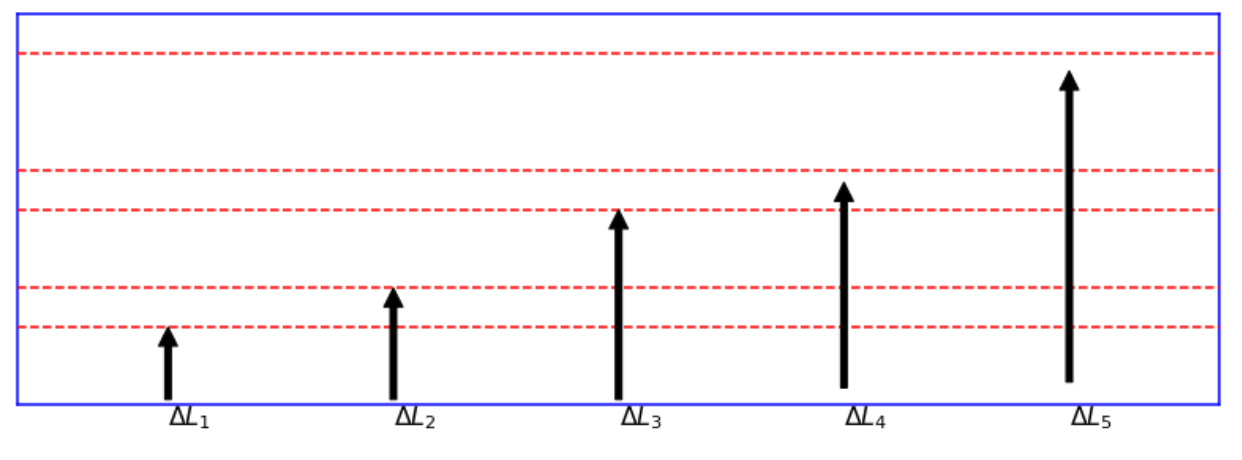
\includegraphics[width=0.95\textwidth]{trajectoire}
		\caption{Trajectoire de la source}
	\end{minipage}
	\begin{minipage}{0.48\textwidth}
		\label{fig:source}
		\centering
		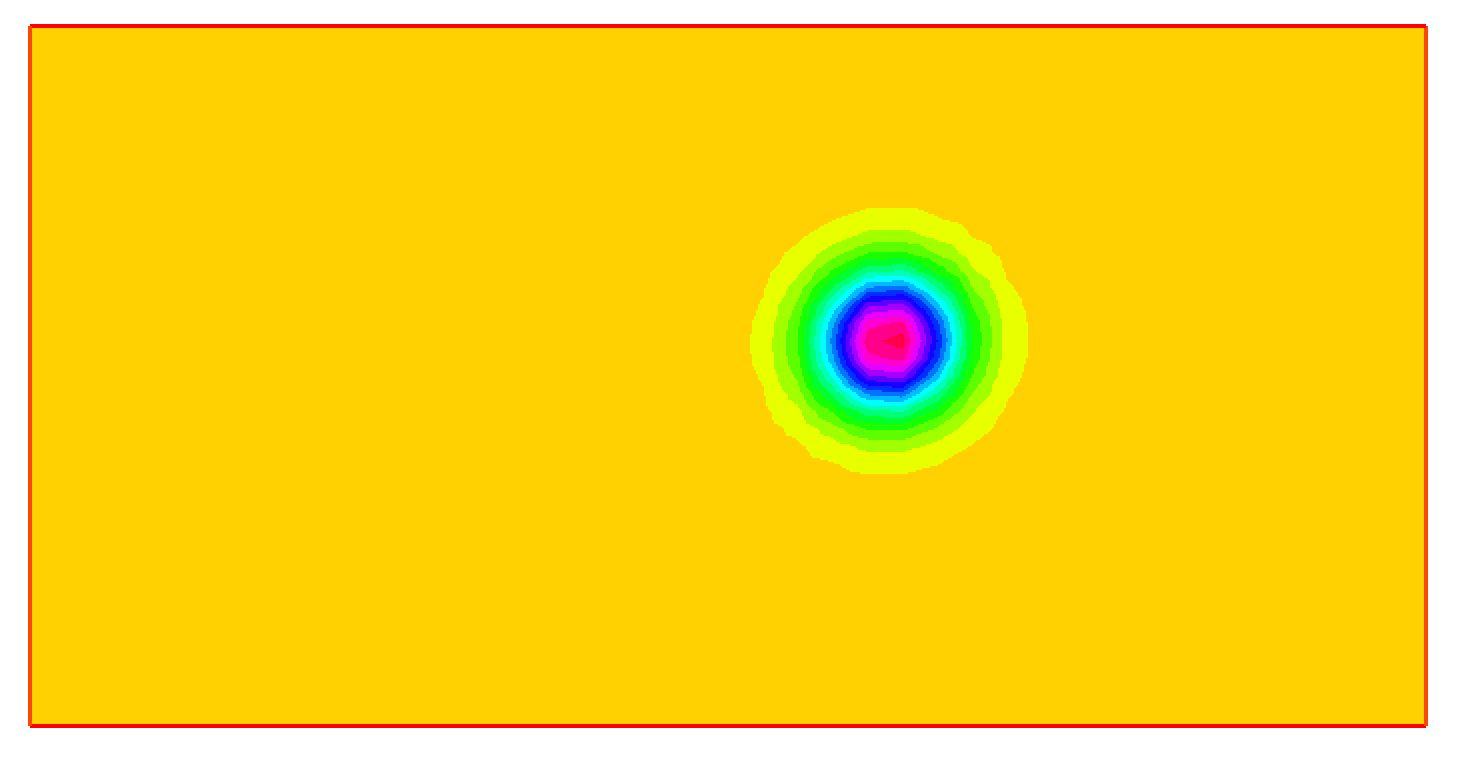
\includegraphics[width=0.8\textwidth]{source}
		\caption{forme de la source}
	\end{minipage}
\end{figure}

On modélise dans un premier temps le temps pour changer de ligne comme nul. Le temps pour effectuer la trajectoire est constant car le nombre de ligne est fixé.
Cette approche induit des discontinuités de trajectoire qui restent simples à gérer (voir ensuite).


\section*{Theorie}
\subsection*{Probleme}

On veut minimiser les endroits n'ayant pas subi de changement phase tout en ne dépassant jamais une valeur seuil de la température ($T_{sup}$), en tout point et en tout instant de fabrication.

Les paramètre d'optimisation sont la distance de chaque ligne $i$ au bord du rectangle $\Delta L_i$. On borne $\Delta L_i$ par 0 et par la largeur de la pièce ($\Delta L\in[0,L_{max}]$). \Math{A revoir pour ces bornes qui ont été changées}
 
\subsection*{Equation de la chaleur}

On pose $\tilde{T}=T-T_{ini}$ (i.e. $T=\tilde{T}+T_{ini}$). On a alors, d'après l'équation \ref{eq:heatEq} (l'arret de la source est modélisée par la fonction source $Q$ elle même. On écrit donc bien l'équation jusqu'à $t_F$ fixé) :

\begin{equation}
\label{eq:ChaleurTilde}
\accDeuxcol{
\Big(\rho\partial_t \tilde{T}+\frac{\lambda}{ep_{car}^2} \tilde{T}-div(\lambda\nabla \tilde{T})\Big)=Q(\Delta L,\tilde{s})& \textrm{in\,}(0,t_F))\times D \\
\tilde{T}=0 & \textrm{in\,}(0,t_F)\times \Gamma_D \\
\tilde{T}(0)=0 & \textrm{in} \Omega
}
\end{equation}




Le problème variationnel lié à la chaleur est alors le suivant :

trouver $\tilde{T}\in V=\{w\in H^1([0,t_M],\Omega) \textrm{tel\,\,que} \,\,w|_{\Gamma_D}=0\}$ tel que

\begin{equation}
\label{eq:pbVarChaleurTF}
\begin{aligned}
\forall v\in V,\,\forall t\in[0,t_M], \qquad\int_{\Omega}\rho\partial_t \tilde{T}v+\frac{\lambda}{ep_{car}^2} \tilde{T}v dx+\int_{\Omega}\lambda\nabla \tilde{T}\nabla vdx-\int_{\Omega}Q(\Delta L,\tilde{s})vdx=0
\end{aligned} 
\end{equation}

\subsection*{Changement de phase}
On souhaite ici que :

\begin{equation}
\forall x\in\Omega,\qquad \Big[\Big(\|T\|_{\infty}-T_{fu}\Big)^-\Big]^2=0
\end{equation}

On approxime la norme infinie par une norme $r$ et on a donc la fonction objectif suivante :

\begin{equation}
J(\Delta L,\tilde{s})=\int_{\Omega}\Bigg[\Bigg(\Big(\int_{0}^{t_F}|T|^rdt\Big)^{\frac{1}{r}}-T_{fu}\Bigg)^-\Bigg]^2=\int_{\Omega}\Bigg[\Bigg(\Big(\int_{0}^{t_M}|\tilde{T}+T_{ini}|^rdt\Big)^{\frac{1}{r}}-T_{fu}\Bigg)^-\Bigg]^2
\end{equation}

\subsection*{Contrainte}
On veut éviter que la température dépasse une température seuil $T_{sup}$. On impose pour cela une contrainte :

\begin{equation}
\label{eq:contrainte}
C(\Delta L,\tilde{s})=\int_{0}^{t_F}\int_{\Omega}[(T-T_{sup})^+]^2dxdt-\textrm{tol}_{sup}=\int_{0}^{t_M}\int_{\Omega}[(\tilde{T}+T_{ini}-T_{sup})^+]^2dxdt-\textrm{tol}_{sup}
\end{equation} 


\subsection*{Source}
On note $t$ le temps ($t=\Delta t*\textrm{it}$), $t_{Li}$ le temps pour parcourir une ligne, $V$ la vitesse de parcours, $(x_C(t),y_C(t,\Delta L))$ le "centre de la gaussienne" à l'instant $t$. On peut alors modéliser l'abscisse et l'ordonnée de la source comme suit :
 On a alors :

\begin{equation}
\begin{aligned}
&x_C(t)=x_{M0}+\Big(t-\textrm{Ent}\Big[\frac{t}{t_{Li}}\Big]*t_{Li}\Big) \\
&Y_C(T)=y_{M0}+\heavi\left(t<t{Li}\right)*\Delta L_{1}+\sum_{i=2}^{nb_{Ligne}}\heavi\left(t\geq(i-1)t_{Li}\right)\heavi\left(t<i*t_{Li}\right)\Delta L_{i}
\end{aligned}
\end{equation}

On a alors la fonction source $Q(t,x,y,\Delta L)=P\exp\bigg(-100\Big(\big(x-x_C(t)\big)^2+\big(y-y_C(t,\Delta L)\big)^2\Big)\bigg)$


\subsection*{Problème d'optimisation}

On s'intéresse donc au problème suivant :

\begin{equation*}
\label{eq:pbOptim}
\begin{aligned}
\min_{\begin{array}{l}
	\Delta L\in[0,L_{max}] \\
	\tilde{s}\in [0,S_{max}]
	\end{array}} J(\Delta L,\tilde{s})=\int_{\Omega}\Bigg[\Bigg(\Big(\int_{0}^{t_F}|\tilde{T}+T_{ini}|^rdt\Big)^{\frac{1}{r}}-T_{fu}\Bigg)^-\Bigg]^2 \\
\\
\textrm{tel\,\,que\quad} C(\Delta L,\tilde{s})=\int_{0}^{t_F}\int_{\Omega}[(\tilde{T}+T_{ini}-T_{sup})^+]^2dxdt-\textrm{tol}_{sup}\leq 0
\end{aligned}
\end{equation*}

avec $\tilde T$ solution de l'Equation \ref{eq:ChaleurTilde}.

\vspace{0cm}

\subsubsection*{Algorithme du Lagrangien}

On va tout d'abord tester l'algorithme d'Uzawa pour gérer la contrainte. On pose $\textrm{lag}_{sup}$ le multiplicateur de Lagrange. On s'intéresse au problème modifié :

\begin{equation}
\min_{\begin{array}{l}
	\Delta L\in[0,L_{max}] \\
	\tilde{s}\in [0,S_{max}]
	\end{array}} J(\Delta L,\tilde{s})
\end{equation}

avec 
\begin{equation}
\tilde{J}(\Delta L,\tilde{s})=\int_{\Omega}\Bigg[\Bigg(\Big(\int_{0}^{t_F}|\tilde{T}+T_{ini}|^rdt\Big)^{\frac{1}{r}}-T_{fu}\Bigg)^-\Bigg]^2+\textrm{lag}_{sup} \Bigg[\int_{0}^{t_F}\int_{\Omega}[(\tilde{T}+T_{ini}-T_{sup})^+]^2dxdt-\textrm{tol}_{sup}\Bigg]
\end{equation}

et on aura a chaque itération 
\begin{equation}
\textrm{lag}_{sup}^{n+1}=\left\{
\begin{array}{ll}
0 & \textrm{si\,\,}C(\Delta L^n)\leq0 \\
\textrm{lag}_{sup}^n+\mu_{lag}C(\Delta L^n,\tilde{s}^n) & \textrm{si\,\,}C(\Delta L^n,\tilde{s}^n)>0
\end{array}
\right.
\end{equation}

\subsubsection*{Augmented Lagrangian Method (ALM)}

Le deuxième algorithme testé est celui du Lagrangien augmenté (ALM dans la suite). (VOIR NOCEDAL XXX)

On pose 
\begin{equation}
\psi(c,\lambda;\mu)=\left\{\begin{array}{ll}
-\lambda*c+\frac{1}{2\mu}*c^2 & \textrm{si\,\,}c-\lambda*\mu\leq 0\\
-\frac{\mu}{2}\lambda^2 & \textrm{sinon}
\end{array}\right.
\end{equation}

On a alors, avec $\lambda$ paramètre à mettre à jour et $\mu$ paramètre de pénalisation fixé, une nouvelle fonction objectif du type :

\begin{equation}
\tilde{J}(\Delta L,\tilde{s})=\int_{\Omega}\Bigg[\Bigg(\Big(\int_{0}^{t_F}|\tilde{T}+T_{ini}|^rdt\Big)^{\frac{1}{r}}-T_{fu}\Bigg)^-\Bigg]^2+\psi\left(\textrm{tol}_{sup}-\Bigg[\int_{0}^{t_F}\int_{\Omega}[(\tilde{T}+T_{ini}-T_{sup})^+]^2dxdt\Bigg],\lambda;\mu\right)
\end{equation}




\subsection*{Calcul des dérivées : méthode sans adjoint pour la température}


On veut trouver la dérivée de $\tilde{J}$ par rapport à $\Delta L$ et $\tilde{s}$. On procède alors de la manière suivante :

\subsubsection*{Derivation de la source}

On dérive la source par rapport à $\Delta L_i$ :

\begin{equation}
\left\{
\begin{array}{ll}
\partial_{\Delta L_1} Q=\heavi(t<t_{Li}) &\,\\
\partial_{\Delta L_i} Q=\heavi(t<i*t_{Li})*\heavi(t\geq(i-1)*t_{Li})&\forall i\in\{2,..,nb_{Ligne}\}
\end{array}\right.
\end{equation}

\subsubsection*{Derivation du tout}

$\tilde{J}(\Delta L,\tilde{s})=\tilde{j}(\tilde{T}(\Delta L,\tilde{s}))$. On a donc :

\begin{equation}
\partial_{\Delta L}\tilde{J}(\Delta L,\tilde{s})=\partial_{\tilde{T}}\tilde{j}(\tilde{T}(\Delta L,\tilde{s}))(\partial_{\Delta L}\tilde{T}(\Delta L,\tilde{s}))
\end{equation}

En dérivant l'équation vérifiée par $\tilde{T}$ en fonction de $\Delta L$, on obtient l'équation vérifiée par $\partial_{\Delta L}\tilde{T}$ :

\begin{equation}
\label{eq:ChaleurDerTilde}
\accDeuxcol{
	\Big(\rho\partial_t \partial_{\Delta L}\tilde{T}+\frac{\lambda}{ep_{car}^2} \partial_{\Delta L}\tilde{T}-div(\lambda\nabla \partial_{\Delta L}\tilde{T})\Big)=\partial_{\Delta L}Q(\Delta L,\tilde{s})& \textrm{in\,}(0,t_F))\times D \\
	\partial_{\Delta L}\tilde{T}=0 & \textrm{in\,}(0,t_F)\times \Gamma_D \\
	\partial_{\Delta L}\tilde{T}(0)=0 & \textrm{in} \Omega
}
\end{equation}

et le problème variationnel associé ainsi que sa discrétisation en temps sont similaires à ceux liés à $\tilde{T}$.

On a aussi accès à la dérivée de la fonction objectif de changement de phase par rapport à $\tilde{T}$ :

\begin{equation}
\partial_{\tilde{T}}J(\tilde{T})(\phi)= \bigint_{\Omega}2\Bigg(\Big(\int_{0}^{t_F}|\tilde{T}+T_{ini}|^rdt\Big)^{\frac{1}{r}}-T_{fu}\Bigg)^-\frac{1}{r}\Big(\int_{0}^{t_F}|\tilde{T}+T_{ini}|^rdt\Big)^{\frac{1}{r}-1}\int_{0}^{t_F}r|\tilde{T}+T_{ini}|^{r-1}\phi dtdx 
\end{equation}

De même, on a accès à la dérivée de la contrainte par rapport à $\tilde{T}$ :

\begin{equation}
\partial_{\tilde{T}}C(\tilde{T})(\phi)= \int_{0}^{t_F}\int_{\Omega}2[(\tilde{T}+T_{ini}-T_{sup})^+]\phi dxdt
\end{equation}

\begin{itemize}
	\item Algorithme d'Uzawa : On obtient alors la dérivée de la fonction objectif par rapport à $\tilde{T}$:
	
	\begin{equation}
	\partial_{\tilde{T}}\tilde{j}(\tilde{T})(\phi)= \partial_{\tilde{T}}J(\Delta L,\tilde{s})(\phi)+ \textrm{lag}_{sup} \partial_{\tilde{T}}C(\Delta L,\tilde{s})(\phi)
	\end{equation}
	et donc la dérivée pour $\tilde{J}$ par rapport à $\Delta L$ :
	
	\begin{equation}
	\partial_{\Delta L}\tilde{J}= \partial_{\tilde{T}}J(\Delta L,\tilde{s})(\partial_{\Delta L}\tilde{T})+ \textrm{lag}_{sup} \partial_{\tilde{T}}C(\Delta L,\tilde{s})(\partial_{\Delta L}\tilde{T})
	\end{equation}
	
	\item ALM : On obtient alors la dérivée de la fonction objectif par rapport à $\tilde{T}$:
	
	\begin{equation}
	\partial_{\tilde{T}}\tilde{j}(\tilde{T})(\phi)= \partial_{\tilde{T}}J(\Delta L,\tilde{s})(\phi)+\partial_1\psi\left(\textrm{tol}_{sup}-C(\Delta L,\tilde{s}),\lambda;\mu\right) \partial_{\tilde{T}}C(\Delta L,\tilde{s})(\phi)
	\end{equation}
	et donc la dérivée pour $\tilde{J}$ par rapport à $\Delta L$ :
	
	\begin{equation}
	\partial_{\Delta L}\tilde{J}= \partial_{\tilde{T}}J(\Delta L,\tilde{s})(\partial_{\Delta L}\tilde{T})+ \partial_1\psi\left(\textrm{tol}_{sup}-C(\Delta L,\tilde{s}),\lambda;\mu\right) \partial_{\tilde{T}}C(\Delta L,\tilde{s})(\partial_{\Delta L}\tilde{T})
	\end{equation}
\end{itemize}



\subsection*{Discrétisation temporelle}

On utilise un schéma implicite pour l'équation de la chaleur :

\begin{equation}
\accUnecol{
	\intO \left(\rho+\frac{\lambda}{ep^2_{car}}\Delta t\right)\tilde{T}_{j+1}vdx+\intO \lambda\Delta t \nabla\tilde{T}_{j+1}\nabla vdx-\intO\left(Q_{j+1}\Delta t-\rho\tilde{T}_j\right)vdx=0 \\
	\tilde{T}_0=T_{ini}
}
\end{equation}

\begin{equation}
J(\Delta L,\tilde{s})=\bigint_{\Omega}\Bigg[\Bigg(\Big(\sum_{j=0}^{N_F}\Delta t|\tilde{T_j}+T_{ini}|^r\Big)^{\frac{1}{r}}-T_{fu}\Bigg)^-\Bigg]^2 
\end{equation}


\begin{equation}
C(\Delta L,\tilde{s})=\sum_{j=0}^{N_F}\Delta t\int_{\Omega}[(\tilde{T_j}+T_{ini}-T_{sup})^+]^2dx-\textrm{tol}_{sup}
\end{equation}

\begin{equation}
\partial_{\Delta L}J(\Delta L,\stilde)= \bigint_{\Omega}2\Bigg(\Big(\sum_{j=0}^{N_F}\left(\Delta t|\tilde{T_i}+T_{ini}|^r\right)\Big)^{\frac{1}{r}}-T_{fu}\Bigg)^-\frac{1}{r}\Big(\sum_{j=0}^{N_F}\left(\Delta t|\tilde{T_j}+T_{ini}|^r\right)\Big)^{\frac{1}{r}-1}\sum_{j=0}^{N_F}\Delta t\left(r|\tilde{T_j}+T_{ini}|^{r-1}\partial_{\Delta L} \tilde{T}\right)dx 
\end{equation}

\begin{equation}
\partial_{\stilde}C(\Delta L\stilde)= \sum_{j=0}^{N_F}\Delta t\left(\int_{\Omega}2[(\tilde{T_j}+T_{ini}-T_{sup})^+]\partial_{\stilde} \tilde{T}\right)dx
\end{equation}


\section*{Algorithme}
On pose 
\begin{equation}
\accUnecol{
	Norme^r=\int_{0}^{t_F}|\tilde{T}+T_{ini}|^rdt=\sum_{i=0}^{N_{t_F}}\Delta t |\tilde{T}_i+T_{ini}|^r \\
	\\
	NormeMoins=min(Norme-T_{fu},0) \\	
	}
\end{equation}

Lorsqu'on simule le passage du laser, à chaque itération, on calcule :
\begin{itemize}
	\item la source $Q$ et la température $\tilde{T}$
	\item les dérivées par rapport à $\Delta L$ et $\tilde{s}$ de la source et les dérivées de la température $\partial_{\Delta L}\tilde{T}$ et $\partial_{\tilde{s}}\tilde{T}$
	\item $Norme=Norme+\Delta t |\tilde{T}_i+T_{ini}|^r$
		\item $derPhaseDeltaL=derPhaseDeltaL+\Delta t |\tilde{T}_i+T_{ini}|^{r-1}*\partial_{\Delta L}\tilde{T}$
		\item $derPhaseStilde=derPhaseStilde+\Delta t |\tilde{T}_i+T_{ini}|^{r-1}*\partial_{\tilde{s}}\tilde{T}$	
		\item $Contrainte=Contrainte+\Delta t \int_{\Omega}\left(\left(\tilde{T}+T_{ini}-T_{sup}\right)^+\right)^2dx$
		\item $derSupDeltaL=derSupDeltaL+\Delta t \int_{\Omega}2\left(\tilde{T}+T_{ini}-T_{sup}\right)^+\partial_{\Delta L}\tilde{T}$
		\item $derSupStilde=derSupStilde+\Delta t \int_{\Omega}2\left(\tilde{T}+T_{ini}-T_{sup}\right)^+\partial_{\tilde{s}}\tilde{T}$
\end{itemize}

A la fin de cette simulation, on calcule :

\begin{itemize}
	\item $Norme=(Norme)^{1/r}$
	\item $NormeMoins=min(Norme-T_{fu},0) $
	\item $J=\int_{\Omega}(NormeMoins^2dx)$
	\item $derPhaseDeltaL=\int_{\Omega}2*NormeMoins*Norme^{1-r}*derPhaseDeltaLdx$
	\item $derPhaseStilde=\int_{\Omega}2*NormeMoins*Norme^{1-r}*derPhaseStildedx$
\end{itemize}

\begin{itemize}
	\item Dans le cas de Uzawa : 
		\begin{itemize}
			\item $L=J+Lag*Contrainte$
			\item $\partial_{\Delta L}L=derPhaseDeltaL+Lag*derSupDeltaL$
			\item $\partial_{\tilde{s}}L=derPhaseStilde+Lag*derSupStilde$	
		\end{itemize}
		
	\item Dans le cas de ALM :	
		\begin{itemize}
			\item $L=J+\psi\left(\textrm{tol}_{sup}-Contrainte,Lag,\mu\right)$
			\item $\partial_{\Delta L}L=derPhaseDeltaL+\partial_1\psi\left(\textrm{tol}_{sup}-Contrainte,Lag,\mu\right)derSupDeltaL$
			\item $\partial_{\tilde{s}}L=derPhaseStilde+\partial_1\psi\left(\textrm{tol}_{sup}-Contrainte,Lag,\mu\right)derSupStilde$	
		\end{itemize}
\end{itemize}	



\subsubsection*{Pas de descente} 
\Math{A choisir}
On consière un coefficient pour chaque variable ($coef_{\Delta L},\,coef_{\tilde{s}}$). Il est initialisé à l'écart maximum que peuvent prendre les valeurs divisé par 10 :
\begin{equation}
coef_{Delta L}=\left(\Delta L _{max}-\Delta L_{min}\right)/10
\end{equation}. 
A chaque itération, le pas de descente est calculé de manière à ce que la différence entre l'ancienne valeur et la nouvelle soit de la valeur du coefficient. On aura donc :
\begin{equation}
|\Delta L_{i+1}-\Delta L_{i}|=coef_{\Delta L}
\end{equation}

Ce coefficient est divisé par 5 lorque l'itération est ratée et multiplié par 1.5 lorsque l'itération est réussie.

%\section*{Tests et résultats}
%
%\subsection*{Algorithme d'Uzawa}
%\subsubsection*{Phase seule}
%%Le premier test fait est l'optimisation de la phase seule avec pour objectif la diminution de $\Delta L$ et l'augmentation de $\stilde$. On prend ici :
%%\begin{itemize}
%%	\item $\Delta L_{min}=0.2$ et $\Delta L_{max}=1$
%%	\item $\stilde_{min}=1.1*\textrm{longueurLigne}$ et $\stilde_{max}=\textrm{nbMaxLignes}*\textrm{longueurLigne}$
%%\end{itemize}
%%Deux initialisations sont testées :
%%\begin{itemize}
%%	\item initialisation 1 : $\Delta L=0.6$ et $\stilde=10$
%%	\item initialisation 2 : $\Delta L=0.2$ et $\stilde=\stilde_{min}$
%%\end{itemize}
%%
%%On a les résultats suivant :
%%
%%\begin{itemize}
%%	\item Initialisation 1 :
%%	
%%	\begin{figure}[H]
%%		\begin{minipage}{0.33\textwidth}
%%			\centering
%%			\includegraphics[width=0.8\textwidth]{phase/Ini1/Lagrangien.png}
%%			\caption{Lagrangien $L$}
%%		\end{minipage}
%%		\begin{minipage}{0.33\textwidth}
%%			\centering
%%			\includegraphics[width=0.8\textwidth]{phase/Ini1/Jphase.png}
%%			\caption{Fonction objectif liée à la phase}
%%		\end{minipage}
%%		\begin{minipage}{0.33\textwidth}
%%			\centering
%%			\includegraphics[width=0.8\textwidth]{phase/Ini1/Contrainte.png}
%%			\caption{Contrainte}
%%		\end{minipage}
%%	\end{figure}
%%	
%%	\begin{figure}[H]
%%		\begin{minipage}{0.45\textwidth}
%%			\centering
%%			\includegraphics[width=0.6\textwidth]{phase/Ini1/DeltaL.png}
%%			\caption{Evolution de $\Delta L$}
%%		\end{minipage}
%%		\begin{minipage}{0.45\textwidth}
%%			\centering
%%			\includegraphics[width=0.6\textwidth]{phase/Ini1/stilde.png}
%%			\caption{Evolution de $\stilde$}
%%		\end{minipage}
%%	\end{figure}
%%	
%%	\item Initialisation 2 :
%%	
%%	\begin{figure}[H]
%%		\begin{minipage}{0.33\textwidth}
%%			\centering
%%			\includegraphics[width=0.8\textwidth]{phase/Ini2/Lagrangien.png}
%%			\caption{Lagrangien $L$}
%%		\end{minipage}
%%		\begin{minipage}{0.33\textwidth}
%%			\centering
%%			\includegraphics[width=0.8\textwidth]{phase/Ini2/Jphase.png}
%%			\caption{Fonction objectif liée à la phase}
%%		\end{minipage}
%%		\begin{minipage}{0.33\textwidth}
%%			\centering
%%			\includegraphics[width=0.8\textwidth]{phase/Ini2/Contrainte.png}
%%			\caption{Contrainte}
%%		\end{minipage}
%%	\end{figure}
%%	
%%	\begin{figure}[H]
%%		\begin{minipage}{0.45\textwidth}
%%			\centering
%%			\includegraphics[width=0.6\textwidth]{phase/Ini2/DeltaL.png}
%%			\caption{Evolution de $\Delta L$}
%%		\end{minipage}
%%		\begin{minipage}{0.45\textwidth}
%%			\centering
%%			\includegraphics[width=0.6\textwidth]{phase/Ini2/stilde.png}
%%			\caption{Evolution de $\stilde$}
%%		\end{minipage}
%%	\end{figure}
%%	
%%\end{itemize}
%
%\subsubsection*{Contrainte seule}
%%Le premier test fait est l'optimisation de la contrainte seule avec pour objectif l'augmentation de $\Delta L$ et la diminution de $\stilde$. On prend ici :
%%\begin{itemize}
%%	\item $\Delta L_{min}=0.2$ et $\Delta L_{max}=1$
%%	\item $\stilde_{min}=1.1*\textrm{longueurLigne}$ et $\stilde_{max}=\textrm{nbMaxLignes}*\textrm{longueurLigne}$
%%\end{itemize}
%%Deux initialisations sont testées :
%%\begin{itemize}
%%	\item initialisation 1 : $\Delta L=0.6$ et $\stilde=10$
%%	\item initialisation 2 : $\Delta L=0.2$ et $\stilde=\stilde_{min}$
%%\end{itemize}
%%
%%On a les résultats suivant :
%%
%%\begin{itemize}
%%	\item Initialisation 1 :
%%	
%%	\begin{figure}[H]
%%		\begin{minipage}{0.33\textwidth}
%%			\centering
%%			\includegraphics[width=0.8\textwidth]{tsup/Ini1/Lagrangien.png}
%%			\caption{Lagrangien $L$}
%%		\end{minipage}
%%		\begin{minipage}{0.33\textwidth}
%%			\centering
%%			\includegraphics[width=0.8\textwidth]{tsup/Ini1/Jphase.png}
%%			\caption{Fonction objectif liée à la phase}
%%		\end{minipage}
%%		\begin{minipage}{0.33\textwidth}
%%			\centering
%%			\includegraphics[width=0.8\textwidth]{tsup/Ini1/Contrainte.png}
%%			\caption{Contrainte}
%%		\end{minipage}
%%	\end{figure}
%%	
%%	\begin{figure}[H]
%%		\begin{minipage}{0.45\textwidth}
%%			\centering
%%			\includegraphics[width=0.6\textwidth]{tsup/Ini1/DeltaL.png}
%%			\caption{Evolution de $\Delta L$}
%%		\end{minipage}
%%		\begin{minipage}{0.45\textwidth}
%%			\centering
%%			\includegraphics[width=0.6\textwidth]{tsup/Ini1/stilde.png}
%%			\caption{Evolution de $\stilde$}
%%		\end{minipage}
%%	\end{figure}
%%	
%%	\item Initialisation 2 :
%%	
%%	\begin{figure}[H]
%%		\begin{minipage}{0.33\textwidth}
%%			\centering
%%			\includegraphics[width=0.8\textwidth]{tsup/Ini2/Lagrangien.png}
%%			\caption{Lagrangien $L$}
%%		\end{minipage}
%%		\begin{minipage}{0.33\textwidth}
%%			\centering
%%			\includegraphics[width=0.8\textwidth]{tsup/Ini2/Jphase.png}
%%			\caption{Fonction objectif liée à la phase}
%%		\end{minipage}
%%		\begin{minipage}{0.33\textwidth}
%%			\centering
%%			\includegraphics[width=0.8\textwidth]{tsup/Ini2/Contrainte.png}
%%			\caption{Contrainte}
%%		\end{minipage}
%%	\end{figure}
%%	
%%	\begin{figure}[H]
%%		\begin{minipage}{0.45\textwidth}
%%			\centering
%%			\includegraphics[width=0.6\textwidth]{tsup/Ini2/DeltaL.png}
%%			\caption{Evolution de $\Delta L$}
%%		\end{minipage}
%%		\begin{minipage}{0.45\textwidth}
%%			\centering
%%			\includegraphics[width=0.6\textwidth]{tsup/Ini2/stilde.png}
%%			\caption{Evolution de $\stilde$}
%%		\end{minipage}
%%	\end{figure}
%%	
%%\end{itemize}
%
%
%
%\subsubsection*{Objectif et contrainte}
%Il est difficile d'obtenir des résultats propres car les dérivées en jeu ont des valeurs assez diverses et il difficile de trouver un pas de descente correct pour faire fonctionner l'algorithme d'Uzawa. Les essais ont donc été abandonnés ici au profit du Lagrangien Augmenté.
%
%
%\subsection*{Augmented Lagrangian Method}
%\newcommand\FichierALM{/Users/mathilde/These/Projets/OptimisationTrajectoire/LignesDroites/NbLignesNonFixe/LignesEquidistantes/deuxVariables/SansAdjoint/Rectangle/AugmentedLagrangian/ResultatsTests/Tout/}
%
%Les tests sont donc faits pour une optimisation simultanée de l'objectif de changement de phase et de réduction de la contrainte.
%
%\paragraph{Initialisation 1 :}
%
%\begin{itemize}
%	\item valeurs initiales : $\Delta L=0.6$ et $\stilde=10$
%	\item parametres d'optimisation : $Lag_{ini}=0$; $\mu=10$; $\textrm{tol}_{sup}=650$
%	\item parametres physiques : $Tini=30;\,Tphase=500;\,Tsup=750$ et $epCaracCoucheCarre=0.0001;$
%\end{itemize}
%
%Le résultat final est :
%\begin{itemize}
%	\item $\Delta L= 0.26235 ;\quad \stilde=15.5214$
%	\item $J_{phase}=9391.72;\quad C= 663.527$
%\end{itemize}
%
%L'évolution en fonction des itérations de chaque grandeur est présentée dans les figures suivantes :
%
%\begin{figure}[H]
%	\begin{minipage}{0.45\textwidth}
%		\centering
%		\includegraphics[width=0.7\textwidth]{\FichierALM/Ini1/DeltaL.png}
%	\end{minipage}
%	\begin{minipage}{0.45\textwidth}
%		\centering
%		\includegraphics[width=0.7\textwidth]{\FichierALM/Ini1/stilde.png}
%	\end{minipage}	
%\end{figure}
%
%\begin{figure}[H]
%	\begin{minipage}{0.45\textwidth}
%		\centering
%		\includegraphics[width=0.7\textwidth]{\FichierALM/Ini1/Jphase.png}
%	\end{minipage}
%	\begin{minipage}{0.45\textwidth}
%		\centering
%		\includegraphics[width=0.7\textwidth]{\FichierALM/Ini1/Contrainte.png}
%	\end{minipage}	
%\end{figure}
%
%\newcounter{x}
%\setcounter{x}{0}
%
%\multido {\n=1+4}{7}{
%	\begin{figure}[H]
%		\begin{minipage}{0.24\textwidth}
%			\addtocounter{x}{\n}
%			\centering
%			\ifnum\thex<10
%				\includegraphics[width=0.9\textwidth]{\FichierALM/Ini1/Xsolide/Xsolide00\thex00.png}
%			\fi
%			\ifnum\thex>9
%				\includegraphics[width=0.9\textwidth]{\FichierALM/Ini1/Xsolide/Xsolide0\thex00.png}
%			\fi
%			\caption*{Iteration \thex}
%		\end{minipage}
%		\begin{minipage}{0.24\textwidth}
%			\addtocounter{x}{1}
%			\centering
%			\ifnum\thex<10
%			\includegraphics[width=0.9\textwidth]{\FichierALM/Ini1/Xsolide/Xsolide00\thex00.png}
%			\fi
%			\ifnum\thex>9
%			\includegraphics[width=0.9\textwidth]{\FichierALM/Ini1/Xsolide/Xsolide0\thex00.png}
%			\fi
%			\caption*{Iteration \thex}
%		\end{minipage}
%		\begin{minipage}{0.24\textwidth}
%			\addtocounter{x}{1}
%			\centering
%			\ifnum\thex<10
%			\includegraphics[width=0.9\textwidth]{\FichierALM/Ini1/Xsolide/Xsolide00\thex00.png}
%			\fi
%			\ifnum\thex>9
%			\includegraphics[width=0.9\textwidth]{\FichierALM/Ini1/Xsolide/Xsolide0\thex00.png}
%			\fi
%			\caption*{Iteration \thex}
%		\end{minipage}
%		\begin{minipage}{0.24\textwidth}
%			\addtocounter{x}{1}
%			\centering
%			\ifnum\thex<10
%			\includegraphics[width=0.9\textwidth]{\FichierALM/Ini1/Xsolide/Xsolide00\thex00.png}
%			\fi
%			\ifnum\thex>9
%			\includegraphics[width=0.9\textwidth]{\FichierALM/Ini1/Xsolide/Xsolide0\thex00.png}
%			\fi
%			\caption*{Iteration \thex}
%		\end{minipage}
%		\setcounter{x}{0}			
%	\end{figure}
%}	
%
%
%
%
%\paragraph{Initialisation 2 :}
%
%\begin{itemize}
%	\item valeurs initiales : $\Delta L=0$ et $\stilde=1.1*L_l=2.2$ avec $L_l$ la longueur d'une ligne
%	\item parametres d'optimisation : $Lag_{ini}=0$; $\mu=10$; $\textrm{tol}_{sup}=650$
%	\item parametres physiques : $Tini=30;\,Tphase=500;\,Tsup=750$ et $epCaracCoucheCarre=0.0001;$
%\end{itemize}
%
%Le résultat final est :
%\begin{itemize}
%	\item $\Delta L= 0.15 ;\quad \stilde=6.0934$
%	\item $J_{phase}=158287;\quad C= 1464.82$
%\end{itemize}
%
%Le résultat n'est pas terrible mais l'initialisation était problablement particulièrement non pertinente.
%L'évolution en fonction des itérations de chaque grandeur est présentée dans les figures suivantes :
%
%\begin{figure}[H]
%	\begin{minipage}{0.45\textwidth}
%		\centering
%		\includegraphics[width=0.7\textwidth]{\FichierALM/Ini2/DeltaL.png}
%	\end{minipage}
%	\begin{minipage}{0.45\textwidth}
%		\centering
%		\includegraphics[width=0.7\textwidth]{\FichierALM/Ini2/stilde.png}
%	\end{minipage}	
%\end{figure}
%
%\begin{figure}[H]
%	\begin{minipage}{0.45\textwidth}
%		\centering
%		\includegraphics[width=0.7\textwidth]{\FichierALM/Ini2/Jphase.png}
%	\end{minipage}
%	\begin{minipage}{0.45\textwidth}
%		\centering
%		\includegraphics[width=0.7\textwidth]{\FichierALM/Ini2/Contrainte.png}
%	\end{minipage}	
%\end{figure}
%
%\setcounter{x}{0}
%
%\multido {\n=1+4}{7}{
%	\begin{figure}[H]
%		\begin{minipage}{0.24\textwidth}
%			\addtocounter{x}{\n}
%			\centering
%			\ifnum\thex<10
%			\includegraphics[width=0.9\textwidth]{\FichierALM/Ini2/Xsolide/Xsolide00\thex00.png}
%			\fi
%			\ifnum\thex>9
%			\includegraphics[width=0.9\textwidth]{\FichierALM/Ini2/Xsolide/Xsolide0\thex00.png}
%			\fi
%			\caption*{Iteration \thex}
%		\end{minipage}
%		\begin{minipage}{0.24\textwidth}
%			\addtocounter{x}{1}
%			\centering
%			\ifnum\thex<10
%			\includegraphics[width=0.9\textwidth]{\FichierALM/Ini2/Xsolide/Xsolide00\thex00.png}
%			\fi
%			\ifnum\thex>9
%			\includegraphics[width=0.9\textwidth]{\FichierALM/Ini2/Xsolide/Xsolide0\thex00.png}
%			\fi
%			\caption*{Iteration \thex}
%		\end{minipage}
%		\begin{minipage}{0.24\textwidth}
%			\addtocounter{x}{1}
%			\centering
%			\ifnum\thex<10
%			\includegraphics[width=0.9\textwidth]{\FichierALM/Ini2/Xsolide/Xsolide00\thex00.png}
%			\fi
%			\ifnum\thex>9
%			\includegraphics[width=0.9\textwidth]{\FichierALM/Ini2/Xsolide/Xsolide0\thex00.png}
%			\fi
%			\caption*{Iteration \thex}
%		\end{minipage}
%		\begin{minipage}{0.24\textwidth}
%			\addtocounter{x}{1}
%			\centering
%			\ifnum\thex<10
%			\includegraphics[width=0.9\textwidth]{\FichierALM/Ini2/Xsolide/Xsolide00\thex00.png}
%			\fi
%			\ifnum\thex>9
%			\includegraphics[width=0.9\textwidth]{\FichierALM/Ini2/Xsolide/Xsolide0\thex00.png}
%			\fi
%			\caption*{Iteration \thex}
%		\end{minipage}
%		\setcounter{x}{0}			
%	\end{figure}
%}	
%
%\paragraph{Initialisation 3 :}
%
%\begin{itemize}
%	\item valeurs initiales : $\Delta L=0.2$ et $\stilde=1.1*L_l=2.2$ avec $L_l$ la longueur d'une ligne
%	\item parametres d'optimisation : $Lag_{ini}=0$; $\mu=10$; $\textrm{tol}_{sup}=650$
%	\item parametres physiques : $Tini=30;\,Tphase=500;\,Tsup=750$ et $epCaracCoucheCarre=0.0001;$
%\end{itemize}
%
%Le résultat final est :
%\begin{itemize}
%	\item $\Delta L= 0.307939 ;\quad \stilde=10.2199$
%	\item $J_{phase}=10254.4;\quad C= 671.638$
%\end{itemize}
%
%Le résultat est à peu près similaire à celui de l'initialisation 1.
%L'évolution en fonction des itérations de chaque grandeur est présentée dans les figures suivantes :
%
%\begin{figure}[H]
%	\begin{minipage}{0.45\textwidth}
%		\centering
%		\includegraphics[width=0.7\textwidth]{\FichierALM/Ini3/DeltaL.png}
%	\end{minipage}
%	\begin{minipage}{0.45\textwidth}
%		\centering
%		\includegraphics[width=0.7\textwidth]{\FichierALM/Ini3/stilde.png}
%	\end{minipage}	
%\end{figure}
%
%\begin{figure}[H]
%	\begin{minipage}{0.45\textwidth}
%		\centering
%		\includegraphics[width=0.7\textwidth]{\FichierALM/Ini3/Jphase.png}
%	\end{minipage}
%	\begin{minipage}{0.45\textwidth}
%		\centering
%		\includegraphics[width=0.7\textwidth]{\FichierALM/Ini3/Contrainte.png}
%	\end{minipage}	
%\end{figure}
%
%\setcounter{x}{0}
%
%\multido {\n=1+4}{7}{
%	\begin{figure}[H]
%		\begin{minipage}{0.24\textwidth}
%			\addtocounter{x}{\n}
%			\centering
%			\ifnum\thex<10
%			\includegraphics[width=0.9\textwidth]{\FichierALM/Ini3/Xsolide/Xsolide00\thex00.png}
%			\fi
%			\ifnum\thex>9
%			\includegraphics[width=0.9\textwidth]{\FichierALM/Ini3/Xsolide/Xsolide0\thex00.png}
%			\fi
%			\caption*{Iteration \thex}
%		\end{minipage}
%		\begin{minipage}{0.24\textwidth}
%			\addtocounter{x}{1}
%			\centering
%			\ifnum\thex<10
%			\includegraphics[width=0.9\textwidth]{\FichierALM/Ini3/Xsolide/Xsolide00\thex00.png}
%			\fi
%			\ifnum\thex>9
%			\includegraphics[width=0.9\textwidth]{\FichierALM/Ini3/Xsolide/Xsolide0\thex00.png}
%			\fi
%			\caption*{Iteration \thex}
%		\end{minipage}
%		\begin{minipage}{0.24\textwidth}
%			\addtocounter{x}{1}
%			\centering
%			\ifnum\thex<10
%			\includegraphics[width=0.9\textwidth]{\FichierALM/Ini3/Xsolide/Xsolide00\thex00.png}
%			\fi
%			\ifnum\thex>9
%			\includegraphics[width=0.9\textwidth]{\FichierALM/Ini3/Xsolide/Xsolide0\thex00.png}
%			\fi
%			\caption*{Iteration \thex}
%		\end{minipage}
%		\begin{minipage}{0.24\textwidth}
%			\addtocounter{x}{1}
%			\centering
%			\ifnum\thex<10
%			\includegraphics[width=0.9\textwidth]{\FichierALM/Ini3/Xsolide/Xsolide00\thex00.png}
%			\fi
%			\ifnum\thex>9
%			\includegraphics[width=0.9\textwidth]{\FichierALM/Ini3/Xsolide/Xsolide0\thex00.png}
%			\fi
%			\caption*{Iteration \thex}
%		\end{minipage}
%		\setcounter{x}{0}			
%	\end{figure}
%}	
%
%\paragraph{Initialisation 4 :}
%
%\begin{itemize}
%	\item valeurs initiales : $\Delta L=\Delta L_{max}=1$ et $\stilde=11*L_l=22$ avec $L_l$ la longueur d'une ligne
%	\item parametres d'optimisation : $Lag_{ini}=0$; $\mu=10$; $\textrm{tol}_{sup}=650$
%	\item parametres physiques : $Tini=30;\,Tphase=500;\,Tsup=750$ et $epCaracCoucheCarre=0.0001;$
%\end{itemize}
%
%Le résultat final est :
%\begin{itemize}
%	\item $\Delta L= 0.311886;\quad \stilde=16.0997$
%	\item $J_{phase}=10874.6;\quad C= 675.787$
%\end{itemize}
%
%On retouve là encore les résultats précédent.
%L'évolution en fonction des itérations de chaque grandeur est présentée dans les figures suivantes :
%
%\begin{figure}[H]
%	\begin{minipage}{0.45\textwidth}
%		\centering
%		\includegraphics[width=0.7\textwidth]{\FichierALM/Ini4/DeltaL.png}
%	\end{minipage}
%	\begin{minipage}{0.45\textwidth}
%		\centering
%		\includegraphics[width=0.7\textwidth]{\FichierALM/Ini4/stilde.png}
%	\end{minipage}	
%\end{figure}
%
%\begin{figure}[H]
%	\begin{minipage}{0.45\textwidth}
%		\centering
%		\includegraphics[width=0.7\textwidth]{\FichierALM/Ini4/Jphase.png}
%	\end{minipage}
%	\begin{minipage}{0.45\textwidth}
%		\centering
%		\includegraphics[width=0.7\textwidth]{\FichierALM/Ini4/Contrainte.png}
%	\end{minipage}	
%\end{figure}
%
%\setcounter{x}{0}
%
%\multido {\n=1+4}{7}{
%	\begin{figure}[H]
%		\begin{minipage}{0.24\textwidth}
%			\addtocounter{x}{\n}
%			\centering
%			\ifnum\thex<10
%			\includegraphics[width=0.9\textwidth]{\FichierALM/Ini4/Xsolide/Xsolide00\thex00.png}
%			\fi
%			\ifnum\thex>9
%			\includegraphics[width=0.9\textwidth]{\FichierALM/Ini4/Xsolide/Xsolide0\thex00.png}
%			\fi
%			\caption*{Iteration \thex}
%		\end{minipage}
%		\begin{minipage}{0.24\textwidth}
%			\addtocounter{x}{1}
%			\centering
%			\ifnum\thex<10
%			\includegraphics[width=0.9\textwidth]{\FichierALM/Ini4/Xsolide/Xsolide00\thex00.png}
%			\fi
%			\ifnum\thex>9
%			\includegraphics[width=0.9\textwidth]{\FichierALM/Ini4/Xsolide/Xsolide0\thex00.png}
%			\fi
%			\caption*{Iteration \thex}
%		\end{minipage}
%		\begin{minipage}{0.24\textwidth}
%			\addtocounter{x}{1}
%			\centering
%			\ifnum\thex<10
%			\includegraphics[width=0.9\textwidth]{\FichierALM/Ini4/Xsolide/Xsolide00\thex00.png}
%			\fi
%			\ifnum\thex>9
%			\includegraphics[width=0.9\textwidth]{\FichierALM/Ini4/Xsolide/Xsolide0\thex00.png}
%			\fi
%			\caption*{Iteration \thex}
%		\end{minipage}
%		\begin{minipage}{0.24\textwidth}
%			\addtocounter{x}{1}
%			\centering
%			\ifnum\thex<10
%			\includegraphics[width=0.9\textwidth]{\FichierALM/Ini4/Xsolide/Xsolide00\thex00.png}
%			\fi
%			\ifnum\thex>9
%			\includegraphics[width=0.9\textwidth]{\FichierALM/Ini4/Xsolide/Xsolide0\thex00.png}
%			\fi
%			\caption*{Iteration \thex}
%		\end{minipage}
%		\setcounter{x}{0}			
%	\end{figure}
%}	
%
%
%
%
%
%
%\section*{Variation : lignes parcourues dans un sens puis dans l'autre}
%
%On s'intéresse maintenant au cas où, au lieu de recommencer toujours de la gauche les lignes droites, on alterne en recommençant du côté où l'on s'est arrêté. Il s'agit alors de reprogrammer la source et de déterminer sa dérivée. 
%
%
%On détermine l'évolution de l'abscisse et de l'ordonnée au cours du temps :
%
%\begin{equation}
%\left\{
%\begin{array}{l}
%\left\{\begin{array}{ll}
%x_C(t)=x_{M0}+\Big(t-\textrm{Ent}\Big[\frac{t}{t_{Li}}\Big]*t_{Li}\Big)*V & \textrm{si\,}\textrm{Ent}\Big[\frac{t}{t_{Li}}\Big]\textrm{\,pair} \\
%x_C(t)=x_{M1}-\Big(t-\textrm{Ent}\Big[\frac{t}{t_{Li}}\Big]*t_{Li}\Big)*V & \textrm{si\,}\textrm{Ent}\Big[\frac{t}{t_{Li}}\Big]\textrm{\,impair}
%\end{array}
%\right. \\
%y_C(T)=\textrm{Ent}\Big[\frac{t}{t_{Li}}\Big]*\Delta L
%\end{array}
%\right. 
%\end{equation}
%
%
%On a alors 
%
%\begin{equation}
%Q(t,x,y,\Delta L,\tilde{s})=S(t,x,y,\Delta L)*\heavi(\tilde{s}-tV)
%\end{equation}  
%
%\subsection*{Résultats}
%\newcommand\FichierALMCh{/Users/mathilde/These/Projets/OptimisationTrajectoire/LignesDroites/NbLignesNonFixe/LignesEquidistantes/deuxVariables/SansAdjoint/RectangleChangementSens/AugmentedLagrangian/ResultatsTests/tout/}
%
%Les initialisations 1 et 3 ont été testées dans ce cas.
%
%\paragraph{Initialisation 1 :}
%
%\begin{itemize}
%	\item valeurs initiales : $\Delta L=0.6$ et $\stilde=10$
%	\item parametres d'optimisation : $Lag_{ini}=0$; $\mu=10$; $\textrm{tol}_{sup}=650$
%	\item parametres physiques : $Tini=30;\,Tphase=500;\,Tsup=750$ et $epCaracCoucheCarre=0.0001;$
%\end{itemize}
%
%Le résultat final est :
%\begin{itemize}
%	\item $\Delta L= 0.339235;\quad \stilde=14.2642 $
%	\item $J_{phase}=20179.4;\quad C= 668.705$
%\end{itemize}
%
%L'évolution en fonction des itérations de chaque grandeur est présentée dans les figures suivantes :
%
%\begin{figure}[H]
%	\begin{minipage}{0.45\textwidth}
%		\centering
%		\includegraphics[width=0.7\textwidth]{\FichierALMCh/Ini1/DeltaL.png}
%	\end{minipage}
%	\begin{minipage}{0.45\textwidth}
%		\centering
%		\includegraphics[width=0.7\textwidth]{\FichierALMCh/Ini1/stilde.png}
%	\end{minipage}	
%\end{figure}
%
%\begin{figure}[H]
%	\begin{minipage}{0.45\textwidth}
%		\centering
%		\includegraphics[width=0.7\textwidth]{\FichierALMCh/Ini1/Jphase.png}
%	\end{minipage}
%	\begin{minipage}{0.45\textwidth}
%		\centering
%		\includegraphics[width=0.7\textwidth]{\FichierALMCh/Ini1/Contrainte.png}
%	\end{minipage}	
%\end{figure}
%
%\setcounter{x}{0}
%
%\multido {\n=1+4}{7}{
%	\begin{figure}[H]
%		\begin{minipage}{0.24\textwidth}
%			\addtocounter{x}{\n}
%			\centering
%			\ifnum\thex<10
%			\includegraphics[width=0.9\textwidth]{\FichierALMCh/Ini1/Xsolide/Xsolide00\thex00.png}
%			\fi
%			\ifnum\thex>9
%			\includegraphics[width=0.9\textwidth]{\FichierALMCh/Ini1/Xsolide/Xsolide0\thex00.png}
%			\fi
%			\caption*{Iteration \thex}
%		\end{minipage}
%		\begin{minipage}{0.24\textwidth}
%			\addtocounter{x}{1}
%			\centering
%			\ifnum\thex<10
%			\includegraphics[width=0.9\textwidth]{\FichierALMCh/Ini1/Xsolide/Xsolide00\thex00.png}
%			\fi
%			\ifnum\thex>9
%			\includegraphics[width=0.9\textwidth]{\FichierALMCh/Ini1/Xsolide/Xsolide0\thex00.png}
%			\fi
%			\caption*{Iteration \thex}
%		\end{minipage}
%		\begin{minipage}{0.24\textwidth}
%			\addtocounter{x}{1}
%			\centering
%			\ifnum\thex<10
%			\includegraphics[width=0.9\textwidth]{\FichierALMCh/Ini1/Xsolide/Xsolide00\thex00.png}
%			\fi
%			\ifnum\thex>9
%			\includegraphics[width=0.9\textwidth]{\FichierALMCh/Ini1/Xsolide/Xsolide0\thex00.png}
%			\fi
%			\caption*{Iteration \thex}
%		\end{minipage}
%		\begin{minipage}{0.24\textwidth}
%			\addtocounter{x}{1}
%			\centering
%			\ifnum\thex<10
%			\includegraphics[width=0.9\textwidth]{\FichierALMCh/Ini1/Xsolide/Xsolide00\thex00.png}
%			\fi
%			\ifnum\thex>9
%			\includegraphics[width=0.9\textwidth]{\FichierALMCh/Ini1/Xsolide/Xsolide0\thex00.png}
%			\fi
%			\caption*{Iteration \thex}
%		\end{minipage}
%		\setcounter{x}{0}			
%	\end{figure}
%}	
%
%
%
%\paragraph{Initialisation 3 :}
%
%\begin{itemize}
%	\item valeurs initiales : $\Delta L=0.2$ et $\stilde=1.1*L_l=2.2$ avec $L_l$ la longueur d'une ligne
%	\item parametres d'optimisation : $Lag_{ini}=0$; $\mu=10$; $\textrm{tol}_{sup}=650$
%	\item parametres physiques : $Tini=30;\,Tphase=500;\,Tsup=750$ et $epCaracCoucheCarre=0.0001;$
%\end{itemize}
%
%Le résultat final est :
%\begin{itemize}
%	\item $\Delta L= 0.30789 ;\quad \stilde=10.2191$
%	\item $J_{phase}=10243.9;\quad C= 663.754$
%\end{itemize}
%
%Le résultat est à peu près similaire à celui de l'initialisation 1.
%L'évolution en fonction des itérations de chaque grandeur est présentée dans les figures suivantes :
%
%\begin{figure}[H]
%	\begin{minipage}{0.45\textwidth}
%		\centering
%		\includegraphics[width=0.7\textwidth]{\FichierALMCh/Ini3/DeltaL.png}
%	\end{minipage}
%	\begin{minipage}{0.45\textwidth}
%		\centering
%		\includegraphics[width=0.7\textwidth]{\FichierALMCh/Ini3/stilde.png}
%	\end{minipage}	
%\end{figure}
%
%\begin{figure}[H]
%	\begin{minipage}{0.45\textwidth}
%		\centering
%		\includegraphics[width=0.7\textwidth]{\FichierALMCh/Ini3/Jphase.png}
%	\end{minipage}
%	\begin{minipage}{0.45\textwidth}
%		\centering
%		\includegraphics[width=0.7\textwidth]{\FichierALMCh/Ini3/Contrainte.png}
%	\end{minipage}	
%\end{figure}
%
%\setcounter{x}{0}
%
%\multido {\n=1+4}{7}{
%	\begin{figure}[H]
%		\begin{minipage}{0.24\textwidth}
%			\addtocounter{x}{\n}
%			\centering
%			\ifnum\thex<10
%			\includegraphics[width=0.9\textwidth]{\FichierALMCh/Ini3/Xsolide/Xsolide00\thex00.png}
%			\fi
%			\ifnum\thex>9
%			\includegraphics[width=0.9\textwidth]{\FichierALMCh/Ini3/Xsolide/Xsolide0\thex00.png}
%			\fi
%			\caption*{Iteration \thex}
%		\end{minipage}
%		\begin{minipage}{0.24\textwidth}
%			\addtocounter{x}{1}
%			\centering
%			\ifnum\thex<10
%			\includegraphics[width=0.9\textwidth]{\FichierALMCh/Ini3/Xsolide/Xsolide00\thex00.png}
%			\fi
%			\ifnum\thex>9
%			\includegraphics[width=0.9\textwidth]{\FichierALMCh/Ini3/Xsolide/Xsolide0\thex00.png}
%			\fi
%			\caption*{Iteration \thex}
%		\end{minipage}
%		\begin{minipage}{0.24\textwidth}
%			\addtocounter{x}{1}
%			\centering
%			\ifnum\thex<10
%			\includegraphics[width=0.9\textwidth]{\FichierALMCh/Ini3/Xsolide/Xsolide00\thex00.png}
%			\fi
%			\ifnum\thex>9
%			\includegraphics[width=0.9\textwidth]{\FichierALMCh/Ini3/Xsolide/Xsolide0\thex00.png}
%			\fi
%			\caption*{Iteration \thex}
%		\end{minipage}
%		\begin{minipage}{0.24\textwidth}
%			\addtocounter{x}{1}
%			\centering
%			\ifnum\thex<10
%			\includegraphics[width=0.9\textwidth]{\FichierALMCh/Ini3/Xsolide/Xsolide00\thex00.png}
%			\fi
%			\ifnum\thex>9
%			\includegraphics[width=0.9\textwidth]{\FichierALMCh/Ini3/Xsolide/Xsolide0\thex00.png}
%			\fi
%			\caption*{Iteration \thex}
%		\end{minipage}
%		\setcounter{x}{0}			
%	\end{figure}
%}	
%
%\section*{Pour la suite}
%
%Plusieurs pistes pour continuer ce projet sont possibles pour la suite :
%
%\begin{itemize}
%	\item Optimisation de la distance entre les lignes pour une trajectoire en lignes droites sur une forme rectangulaire :
%	\begin{itemize}
%		\item Amélioration des données et de la définition des fonctions objectifs et de contraintes pour être au plus près du problème physique.
%		\item Traitement de la contrainte de manière plus forte ou algorithme d'optimisation qui converge plus rapidement. (à voir pour ce point là)
%	\end{itemize}
%	
%	\item Optimisation de la distance entre les lignes pour une trajectoire en lignes droites :
%	\begin{itemize}
%		\item Adaptation à d'autres formes :
%		\begin{itemize}
%			\item formes dont on connait le paramétrage des bords : triangle, ovale, cercle, ... Le problème principal à régler est que la longueur de chaque ligne dépend de $\Delta L$ et on induit de nouvelles discontinuités beaucoup plus compliquées à régler dans la source.
%			\item formes dont on n'a pas d'équation explicite (levelset de fonction, ...)
%		\end{itemize}
%	\end{itemize}
%	
%	\item Trajectoires en lignes droite : ajout d'un angle de parcours et optimisation de l'angle.
%	\begin{itemize}
%		\item en 2D : on le fait pour une seule couche afin de voir si physiquement, ça fait une différence (ça en fait une d'un point de vue vitesse de parcours, cf Rajan 2001)
%		\item en 3D : on construit couche après couche et on veut savoir l'évolution de la distance entre les lignes ainsi que de l'angle pour chaque couche.
%	\end{itemize}
%	
%	\item Adaptation à d'autres types de trajectoires :
%	\begin{itemize}
%		\item zig-zag
%		\item isovaleurs
%		\item ... mais ce qui est sûr, c'est qu'il faudra trouver un moyen de gérer la discontinuité de la source.
%	\end{itemize}
%\end{itemize}
%
%%\section*{Annexe : methode avec adjoint pour la température}
%%
%%\subsection*{Derivation du problème}
%%
%%Afin de déterminer la dérivée, on utilise une méthode adjoint :
%%
%%\begin{equation}
%%\begin{array}{ll}
%%\mathcal{L}(\Delta L,\tilde{s},v,q,\mu)= & \bigint_{\Omega}\Bigg[\Bigg(\Big(\int_{0}^{t_F}|v+T_{ini}|^rdt\Big)^{\frac{1}{r}}-T_{fu}\Bigg)^-\Bigg]^2dx +\textrm{lag}_{sup} \Bigg[\bigint_{0}^{t_F}\bigint_{\Omega}[(v+T_{ini}-T_{sup})^+]^2dxdt-\textrm{tol}_{sup}\Bigg] \\
%%\\
%%\, & + \bigint_{0}^{t_F}\bigint_{\Omega}\rho(\partial_t v)q+\frac{\lambda}{ep_{car}^2} vq-div(\lambda\nabla v)q-Q(\Delta L,\tilde{s})q dxdt +\bigint_{\Omega}\rho v(0)q(0) dx+\bigint_{0}^{t_F}\bigint_{\Gamma_D}\mu v dsdt\\
%%\end{array}
%%\end{equation}
%%
%%d'où 
%%
%%\begin{equation}
%%\begin{array}{ll}
%%\mathcal{L}(\Delta L,\tilde{s},v,q,\mu)= & \bigint_{\Omega}\Bigg[\Bigg(\Big(\int_{0}^{t_F}|v+T_{ini}|^rdt\Big)^{\frac{1}{r}}-T_{fu}\Bigg)^-\Bigg]^2dx +\textrm{lag}_{sup} \Bigg[\bigint_{0}^{t_F}\bigint_{\Omega}[(v+T_{ini}-T_{sup})^+]^2dxdt-\textrm{tol}_{sup}\Bigg] \\
%%\\
%%\, & +\bigint_{\Omega}\rho v(0)q(0) dx+ \bigint_{0}^{t_F}\bigint_{\Omega}\rho\partial_t (vq)dxdt-\bigint_{0}^{t_F}\bigint_{\Omega}\rho(\partial_t q)vdxdt\\
%%\\
%%\, &+\bigint_{0}^{t_F}\bigint_{\Omega}\lambda\nabla v\nabla qdxdt +\bigint_{0}^{t_F}\bigint_{\Omega}\frac{\lambda}{ep_{car}^2} vq-Q(\Delta L,\tilde{s})q dxdt +\bigint_{0}^{t_F}\bigint_{\Gamma_D}\mu v -(\lambda\nabla v)qdsdt\\
%%\end{array}
%%\end{equation}
%%
%%et donc 
%%
%%\begin{equation}
%%\begin{array}{ll}
%%\mathcal{L}(\Delta L,\tilde{s},v,q,\mu)= & \bigint_{\Omega}\Bigg[\Bigg(\Big(\int_{0}^{t_F}|v+T_{ini}|^rdt\Big)^{\frac{1}{r}}-T_{fu}\Bigg)^-\Bigg]^2dx +\textrm{lag}_{sup} \Bigg[\bigint_{0}^{t_F}\bigint_{\Omega}[(v+T_{ini}-T_{sup})^+]^2dxdt-\textrm{tol}_{sup}\Bigg] \\
%%\\
%%\, & +\bigint_{\Omega}\rho v(t_F)q(t_F) dx-\bigint_{0}^{t_F}\bigint_{\Omega}\rho(\partial_t q)vdxdt\\
%%\\
%%\, &+\bigint_{0}^{t_F}\bigint_{\Omega}\lambda\nabla v\nabla qdxdt +\bigint_{0}^{t_F}\bigint_{\Omega}\frac{\lambda}{ep_{car}^2} vq-Q(\Delta L,\tilde{s})q dxdt +\bigint_{0}^{t_F}\bigint_{\Gamma_D}\mu v -(\lambda\nabla v)qdsdt\\
%%\end{array}
%%\end{equation}
%%
%%En dérivant par rapport à $v$ et en appliquant à la solution $\tilde{T}$ de l'équation de la chaleur :
%%
%%\begin{equation}
%%\begin{array}{ll}
%%\partial_v\mathcal{L}&(\Delta L,\tilde{s},\tilde{T},q,\mu)(\phi)= \textrm{lag}_{sup} \bigint_{0}^{t_F}\bigint_{\Omega}2[(\tilde{T}+T_{ini}-T_{sup})^+]\phi dxdt\\
%%\\
%%\,\, +&\bigint_{\Omega}2\Bigg(\Big(\int_{0}^{t_F}|\tilde{T}+T_{ini}|^rdt\Big)^{\frac{1}{r}}-T_{fu}\Bigg)^-\frac{1}{r}\Big(\int_{0}^{t_F}|\tilde{T}+T_{ini}|^rdt\Big)^{\frac{1}{r}-1}\int_{0}^{t_F}r|\tilde{T}+T_{ini}|^{r-1}\phi dtdx \\
%%\\
%%\,\, + &\bigint_{0}^{t_F}\bigint_{\Omega}-\rho\partial_t q \phi+ \frac{\lambda}{ep_{car}^2} \phi q+\lambda\nabla \phi\nabla q dxdt +\bigintO\rho q(t_F)\phi(t_F)dx \\
%%\\
%%\,\, + & \bigint_{0}^{t_F}\bigint_{\Gamma_D}\Big(\mu \phi-(\lambda\nabla \phi)nq \Big)dsdt\\
%%\end{array}
%%\end{equation}
%%
%%
%%\begin{equation}
%%\begin{array}{ll}
%%\partial_v\mathcal{L}&(\Delta L,\tilde{s},\tilde{T},q,\mu)(\phi)= \textrm{lag}_{sup} \bigint_{0}^{t_F}\bigint_{\Omega}2[(\tilde{T}+T_{ini}-T_{sup})^+]\phi dxdt\\
%%\\
%%\,\, +&\bigint_{\Omega}2\Bigg(\Big(\int_{0}^{t_F}|\tilde{T}+T_{ini}|^rdt\Big)^{\frac{1}{r}}-T_{fu}\Bigg)^-\frac{1}{r}\Big(\int_{0}^{t_F}|\tilde{T}+T_{ini}|^rdt\Big)^{\frac{1}{r}-1}\int_{0}^{t_F}r|\tilde{T}+T_{ini}|^{r-1}\phi dtdx \\
%%\\
%%\,\, + &\bigint_{0}^{t_F}\bigint_{\Omega}-\rho\partial_t q \phi+ \frac{\lambda}{ep_{car}^2} \phi q-\textrm{div}\big(\lambda\nabla q\big) \phi dxdt +\bigintO\rho q(t_F)\phi(t_F)dx \\
%%\\
%%\,\, + & \bigint_{0}^{t_F}\bigint_{\Gamma_D}\Big(\mu \phi-(\lambda\nabla \phi)nq-(\lambda\nabla q)n\phi \Big)dsdt\\
%%\end{array}
%%\end{equation}
%%
%%On en déduit alors l'équation des adjoints :
%%
%%\begin{equation}
%%\left\{
%%\begin{array}{ll}
%%\rho\partial_t p-\frac{\lambda}{ep_{car}^2} p+div(\lambda\nabla p)= 2\textrm{lag}_{sup}\textrm{ind}_{Cont}(t)+2\textrm{N}_{Moins}\textrm{N}_r^{1-r}(\textrm{ind}_{Phase}(t))^{r-1}& \textrm{in} (0,t_F)\times \Omega \\
%%p=0 & \textrm{in} (0,t_F)\times \Gamma_D \\
%%p(t_F)= 0 & \textrm{in} \, \Omega \\
%%\mu=(\lambda\nabla q)n & \textrm{in}(0,t_F)\times\Gamma_D
%%\end{array}
%%\right.
%%\end{equation}
%%
%%avec 
%%
%%\begin{equation}
%%\begin{aligned}
%%&\textrm{ind}_{Cont}(t)=(\tilde{T}+T_{ini}-T_{sup})^+ \\
%%&\textrm{ind}_{Phase}(t)=|\tilde{T}+T_{ini}| \\
%%& \textrm{N}_r=\Big(\int_{0}^{t_F}|\tilde{T}+T_{ini}|^rdt\Big)^{\frac{1}{r}}\\
%%&\textrm{N}_{Moins}=(\textrm{Norme}-T_{fu})^-=\Big(\int_{0}^{t_F}|\tilde{T}+T_{ini}|^rdt\Big)^{\frac{1}{r}}-T_{fu}\Big)^-
%%\end{aligned}
%%\end{equation}
%%
%%Et la forme variationnelle suivante : trouver $p\in V$ tel que
%%\begin{equation}
%%\forall \phi\in V, \quad \int_{\Omega}\rho\partial_t p\phi-\lambda\nabla p\nabla \phi-\frac{\lambda}{ep_{car}^2} p \phi -\Big(2\textrm{lag}_{sup}\textrm{ind}_{Cont}(t)+2\textrm{N}_{Moins}\textrm{N}_r^{1-r}(\textrm{ind}_{Phase}(t))^{r-1}\Big)dx=0
%%\end{equation}
%%
%%
%%De plus, on obtient alors la dérivée de la fonction objectif par rapport à $\Delta L$ et $\tilde s$ :
%%
%%\begin{equation}
%%\begin{aligned}
%%&\partial_{\Delta L}\tilde{J}(\Delta L, \tilde s)=-\int_{0}^{t_F}\intO \partial_{\Delta L} Q p dxdt \\
%%&\partial_{\tilde s}\tilde{J}(\Delta L, \tilde s)=-\int_{0}^{t_F}\intO \partial_{\tilde s} Q p dxdt 
%%\end{aligned}
%%\end{equation}
%%
%%avec 
%%\begin{equation}
%%\begin{array}{ll}
%%\partial_{\Delta L} Q&=\heavi(\tilde{s}-tV)S(t,x,y,\Delta L)*(-200)(y-y_C(t,\Delta L))*(-1)*\partial_{\Delta L}y_C(t,\Delta L)\\
%%\\
%%\, & =\heavi(\tilde{s}-tV)S(t,x,y,\Delta L)*(-200)(y-y_C(t,\Delta L))*(-1)*(-1)*\textrm{Ent}\Big[\frac{t}{t_{Li}}\Big] \\
%%\\
%%\, & =\heavi(\tilde{s}-tV)S(t,x,y,\Delta L)*(-200)(y-y_C(t,\Delta L))\textrm{Ent}\Big[\frac{t}{t_{Li}}\Big] 
%%\end{array} 
%%\end{equation}
%%
%%et 
%%
%%\begin{equation}
%%\partial_{\tilde{s} Q}=S(t,x,y,\Delta L)*\heaviP(\tilde{s}-tV)
%%\end{equation}
%%
%%
%%\subsection*{Discrétisation temporelle}
%%
%%On utilise un schéma implicite pour l'équation de la chaleur :
%%
%%\begin{equation}
%%\accUnecol{
%%	\intO \left(\rho+\frac{\lambda}{ep^2_{car}}\Delta t\right)\tilde{T}_{j+1}vdx+\intO \lambda\Delta t \nabla\tilde{T}_{j+1}\nabla vdx-\intO\left(Q_{j+1}\Delta t-\rho\tilde{T}_j\right)vdx=0 \\
%%	\tilde{T}_0=T_{ini}
%%}
%%\end{equation}
%%
%%\begin{equation}
%%J(\Delta L,\tilde{s})=\bigint_{\Omega}\Bigg[\Bigg(\Big(\sum_{j=0}^{N_F}\Delta t|\tilde{T_j}+T_{ini}|^r\Big)^{\frac{1}{r}}-T_{fu}\Bigg)^-\Bigg]^2 
%%\end{equation}
%%
%%
%%\begin{equation}
%%C(\Delta L,\tilde{s})=\sum_{j=0}^{N_F}\Delta t\int_{\Omega}[(\tilde{T_j}+T_{ini}-T_{sup})^+]^2dx-\textrm{tol}_{sup}
%%\end{equation}
%%
%%\begin{equation}
%%\begin{array}{l}
%%\forall \phi\in V, \\
%%\\
%%\accUnecol{
%%	\intO\left(\rho+\frac{\lambda}{ep_{car}^2}\Delta t\right)p_j\phi+\lambda\Delta t\nabla p_j \nabla \phi dx +\bigintO\Delta t\Big(2\textrm{lag}_{sup,j}\textrm{ind}_{Cont,j}+2\textrm{N}_{Moins}\textrm{N}_r^{1-r}(\textrm{ind}_{Phase,j})^{r-1}\Big)\phi-\intO\rho p_{j+1}\phi dx=0 \\
%%	p_{N_F}=0
%%}
%%\end{array}
%%\end{equation}
%%
%%
%%\begin{equation}
%%\begin{aligned}
%%&\partial_{\Delta L}\tilde{J}(\Delta L, \tilde s)=-\sum_{0}^{t_F}\Delta t\intO \partial_{\Delta L} Q_j p dx=-\sum_{0}^{t_F}\Delta t\intO\heavi(\tilde{s}-t_jV)S(t_j,x,y,\Delta L)*(-200)(y-y_C(t_j,\Delta L))\textrm{Ent}\Big[\frac{t_j}{t_{Li}}\Big]p_j dx \\
%%&\partial_{\tilde s}\tilde{J}(\Delta L, \tilde s)=-\sum_{0}^{t_F}\intO \partial_{\tilde s} Q_j p_j dx =-\sum_{0}^{t_F}\intO S(t_j,x,y,\Delta L)*\heaviP(\tilde{s}-t_jV)p_j dx
%%\end{aligned}
%%\end{equation}




\end{document}